% !TeX program = xelatex
% Encoding: UTF-8. Compile twice with XeLaTeX.
\documentclass[UTF8,a4paper,zihao=5,fontset=fandol]{ctexart}
\usepackage[left=21mm,right=21mm,top=20mm,bottom=20mm,headheight=14pt,headsep=6mm,footskip=10mm]{geometry}
\usepackage{amsmath,amssymb,bm,graphicx,booktabs,enumitem,xcolor,fancyhdr,hyperref}
\usepackage{algorithm,algpseudocode}
\floatname{algorithm}{算法}
\renewcommand{\algorithmicrequire}{\textbf{输入：}}
\renewcommand{\algorithmicensure}{\textbf{输出：}}
\definecolor{accent}{HTML}{006B88}
\definecolor{muted}{HTML}{536773}
\hypersetup{colorlinks=true,urlcolor=accent,linkcolor=accent,
  pdftitle={张量网络作业：DMRG 求解自旋 1/2 Heisenberg 链},
  pdfauthor={课程作业：AI 辅助实现与数值验证}}
\graphicspath{{images/}}
\linespread{1.12}
\setlength{\parindent}{2em}
\setlength{\parskip}{3pt}
\setlength{\abovedisplayskip}{7pt}
\setlength{\belowdisplayskip}{7pt}
\setlength{\tabcolsep}{5pt}
\renewcommand{\arraystretch}{1.18}
\setlist[enumerate]{leftmargin=2em,itemsep=3pt,topsep=4pt,parsep=0pt}
\ctexset{
  section={format=\large\bfseries\raggedright,beforeskip=9pt,afterskip=7pt},
  subsection={format=\normalsize\bfseries\raggedright,beforeskip=7pt,afterskip=4pt}}
\pagestyle{fancy}
\fancyhf{}
\fancyhead[L]{\small\color{muted}张量网络作业\quad DMRG / MPS}
\fancyhead[R]{\small\color{muted}2026-10-27}
\fancyfoot[C]{\small\thepage}
\renewcommand{\headrulewidth}{0.3pt}
\newcommand{\avg}[1]{\left\langle #1\right\rangle}
\newcommand{\code}[1]{\texttt{#1}}

\begin{document}
\section*{第一题\quad DMRG 优化 MPS}

\subsection*{模型与约定}
取反铁磁耦合 $J=1$、$\hbar=1$，使用开边界，链首尾不相连：
\[
H=\sum_{i=1}^{L-1}\bm S_i\cdot\bm S_{i+1}
 =\sum_{i=1}^{L-1}
 \left[S_i^zS_{i+1}^z+
 \frac12\left(S_i^+S_{i+1}^-+S_i^-S_{i+1}^+\right)\right],
 \qquad S^\alpha=\frac{\sigma^\alpha}{2}.
\]
用矩阵乘积态（MPS）表示波函数：
\[
|\psi\rangle=
\sum_{s_1,\ldots,s_L} A_1^{s_1}A_2^{s_2}\cdots A_L^{s_L}
|s_1\cdots s_L\rangle,\qquad \chi_i\le m.
\]
其中 $m$ 为每条内部虚键保留态数的上限，靠近边界的实际维数可以更小。

\subsection*{双站点有限 DMRG 算法}
保持局部优化区外的 MPS 为正交规范，解有效基态问题后作 SVD 截断。
全程使用普通稠密张量，不按总 $S^z$ 或 SU(2) 对称性分块。
\begin{algorithm}[H]
\caption{双站点 DMRG 的伪代码}
\footnotesize
\begin{algorithmic}[1]
\Require $L$，递增序列 $\{m\}$，$\tau_E=10^{-9}$，$\tau_{\mathrm{eig}}=10^{-11}$
\Ensure 各 $m$ 的能量 $E(m)$、最终 MPS 与自旋关联
\State 初始化随机归一化乘积态 MPS，随机种子为 $7$
\For{$m\in\{4,8,16,32,64,128\}$}
  \State 以上一步的 MPS 为初态，构造右环境；$E_{\mathrm{prev}}\gets\infty$，$q\gets0$
  \For{$k=1,\ldots,40$}
    \For{方向 $d\in(\text{向右},\text{向左})$}
      \For{按 $d$ 顺序遍历相邻键 $(i,i+1)$}
        \State 合并 $\Theta\gets A_iA_{i+1}$；用左右环境构造 $H_{\mathrm{eff}}$ 的作用
        \State 求 $H_{\mathrm{eff}}\Theta=E_{\mathrm{loc}}\Theta$ 的最低本征态，容差 $\tau_{\mathrm{eig}}$
        \State $U\operatorname{diag}(\lambda)V^\dagger\gets\operatorname{SVD}(\Theta_{(as),(tb)})$
        \State 保留最大的至多 $m$ 个奇异值，并令 $\widetilde\lambda=\lambda_{1:m}/\|\lambda_{1:m}\|$
        \State 按方向分裂 $\Theta$、移动正交中心并更新环境
      \EndFor
    \EndFor
    \State 用截断后的归一化 MPS 计算 $E=\langle\psi|H|\psi\rangle$
    \State 若 $|E-E_{\mathrm{prev}}|<\tau_E$，令 $q\gets q+1$；否则 $q\gets0$
    \If{$k\ge3$ 且 $q\ge2$} \State \textbf{break} \EndIf
    \State $E_{\mathrm{prev}}\gets E$
  \EndFor
  \State 保存 $E(m)$、截断权重和 MPS
\EndFor
\State 逐格点收缩最终 MPS，分别计算 $x,y,z$ 关联并求和
\end{algorithmic}
\end{algorithm}
向右扫描时 $A_i=U_m$、$A_{i+1}=\operatorname{diag}(\widetilde\lambda)V_m^\dagger$；
向左时将奇异值吸收到左张量。局部丢弃权重为
$\epsilon_{\mathrm{disc}}=\sum_{k>m}\lambda_k^2/\sum_k\lambda_k^2$。

\subsection*{程序与运行}
完整程序为 \code{dmrg\_heisenberg.py}，核心函数为
\code{dmrg}、\code{optimize\_pair}、\code{grow\_block}。
用 NumPy / SciPy 完成 DMRG，Matplotlib 绘图：
{\small
\begin{verbatim}
python -m pip install -r requirements.txt
python dmrg_heisenberg.py --validate
python dmrg_heisenberg.py --length 64 --bonds 4 8 16 32 64 128
\end{verbatim}
}
\InputIfFileExists{repository-note.tex}{}{}
{\footnotesize
\noindent 原题：Shoushu Gong，\emph{A brief introduction to tensor network states}
（2026-10-09）第 73 页。算法参考：
\href{https://arxiv.org/abs/1008.3477}{U. Schollw\"ock, Annals of Physics 326, 96--192 (2011)}；
求解器选项见 \href{https://docs.scipy.org/doc/scipy/reference/generated/scipy.sparse.linalg.eigsh.html}{SciPy eigsh 文档}。
}

\clearpage
\section*{第二题\quad 能量随保留态数的变化}
固定 $L=64$，取 $m=4,8,16,32,64,128$，随机种子为 $7$。
各 $m$ 均满足扫描停止标准。表中 $E$ 为总能量，$e=E/64$ 为每格点能量；
最后一列为最后一轮扫描中最大的局部丢弃权重。

\begin{center}
\small
\begin{tabular}{rrrrrr}
\toprule
$m$ & $E(m)$ & $e(m)$ & $E(m)-E(128)$ & 扫描轮数 & $\epsilon_{\mathrm{disc,max}}$\\
\midrule
4 & $-28.02753345529$ & $-0.4379302102$ & $1.479\times10^{-1}$ & 29 & $1.23\times10^{-3}$\\
8 & $-28.16609853027$ & $-0.4400952895$ & $9.326\times10^{-3}$ & 7 & $6.07\times10^{-5}$\\
16 & $-28.17478476399$ & $-0.4402310119$ & $6.401\times10^{-4}$ & 6 & $1.07\times10^{-5}$\\
32 & $-28.17541324514$ & $-0.4402408320$ & $1.161\times10^{-5}$ & 5 & $1.61\times10^{-7}$\\
64 & $-28.17542480834$ & $-0.4402410126$ & $5.131\times10^{-8}$ & 3 & $6.92\times10^{-10}$\\
128 & $-28.17542485965$ & $-0.4402410134$ & 参考值 & 3 & $1.53\times10^{-12}$\\
\bottomrule
\end{tabular}

\vspace{7pt}
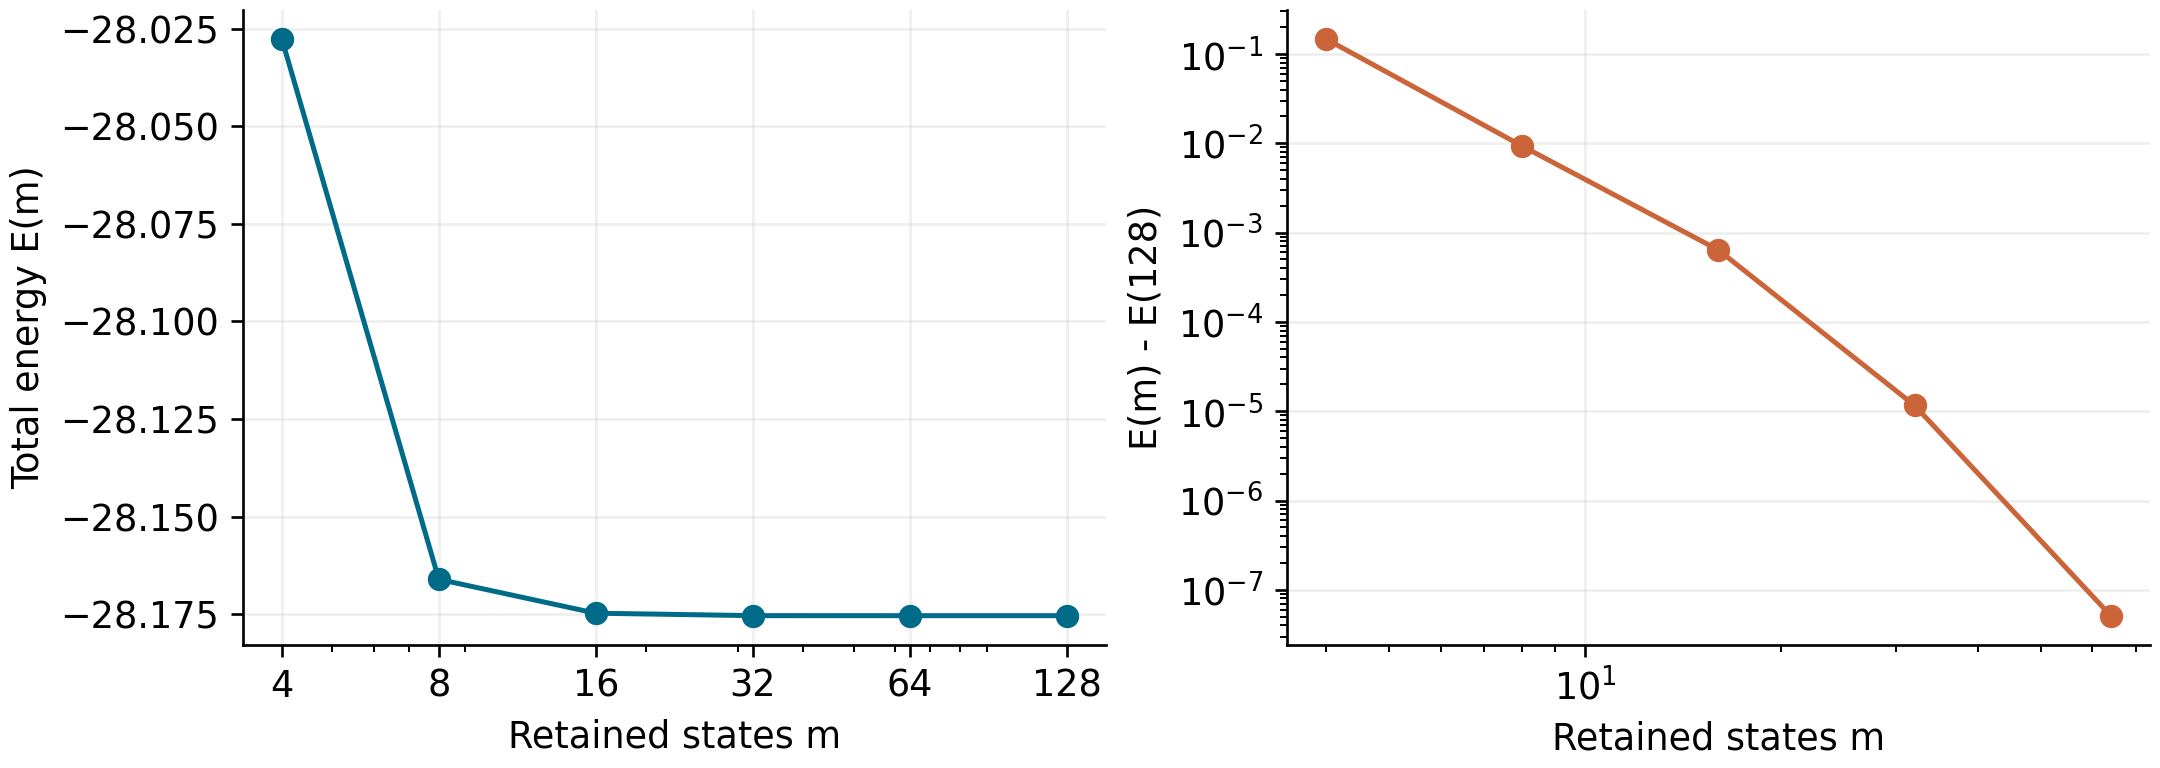
\includegraphics[width=\linewidth]{energy_convergence.png}

{\footnotesize 左：总能量随保留态数的变化。右：相对 $m=128$ 结果的差值，使用双对数坐标。}
\end{center}

\subsection*{数值结论}
$m=128$ 时得到
\[
\boxed{E_0\simeq-28.17542485965},\qquad
\boxed{E_0/L\simeq-0.440241013432}.
\]
随 $m$ 增加，能量逐步降低并趋于稳定。从 $m=64$ 增加到 $128$ 时，
总能量变化约为 $5.13\times10^{-8}$，每格点变化约为 $8.02\times10^{-10}$。

增大 $m$ 扩大 MPS 的表示能力、减小截断影响。
本表以 $E(128)$ 作为数值参照，差值不是严格误差上界；
以上结果对应有限开链，不是热力学极限。

\subsection*{正确性核对}
对 $L=2,4,6,8,10$，在完整的 $2^L$ 维空间进行独立精确对角化。
DMRG 能量最大误差小于 $4.45\times10^{-15}$，
$C^{zz}$ 的最大误差小于 $3.75\times10^{-16}$。
例如，$L=4$ 时 $E=-1.616025403784$；
$L=10$ 时 $E=-4.258035207283$。

对于 $L=64$，由完整关联矩阵计算
$\sum_{i=1}^{63}\avg{\bm S_i\cdot\bm S_{i+1}}$，
与独立计算的能量相差约 $1.17\times10^{-13}$。

\clearpage
\section*{第三题\quad 基态自旋关联函数}
使用 $m=128$ 的基态，格点从 $1$ 编号，固定参考格点 $i=32$：
\[
C^{zz}(r)=\avg{S_{32}^zS_{32+r}^z},\qquad
C(r)=\avg{\bm S_{32}\cdot\bm S_{32+r}}.
\]
逐格点收缩 MPS，在目标格点插入自旋算符，其余格点插入单位算符：
\[
\mathcal E_i^O(X)=
\sum_{s,t}\langle s|O|t\rangle\,(A_i^s)^\dagger X A_i^t.
\]
从标量 $1$ 顺次收缩，以最终范数归一化；同一格点插入算符乘积。
各自旋分量独立计算后相加，没有预先设定 $C=3C^{zz}$。

\begin{center}
\small
\begin{tabular}{rrrr}
\toprule
距离 $r$ & 目标格点 $j$ & $C^{zz}(r)$ & $C(r)$\\
\midrule
0 & 32 & $0.250000000$ & $0.750000000$\\
1 & 33 & $-0.134414761$ & $-0.403244283$\\
2 & 34 & $0.060682958$ & $0.182048874$\\
3 & 35 & $-0.044218924$ & $-0.132656773$\\
4 & 36 & $0.034663112$ & $0.103989336$\\
8 & 40 & $0.018981356$ & $0.056944068$\\
16 & 48 & $0.010088427$ & $0.030265284$\\
24 & 56 & $0.006646063$ & $0.019938186$\\
32 & 64 & $0.003850496$ & $0.011551489$\\
\bottomrule
\end{tabular}

\vspace{6pt}
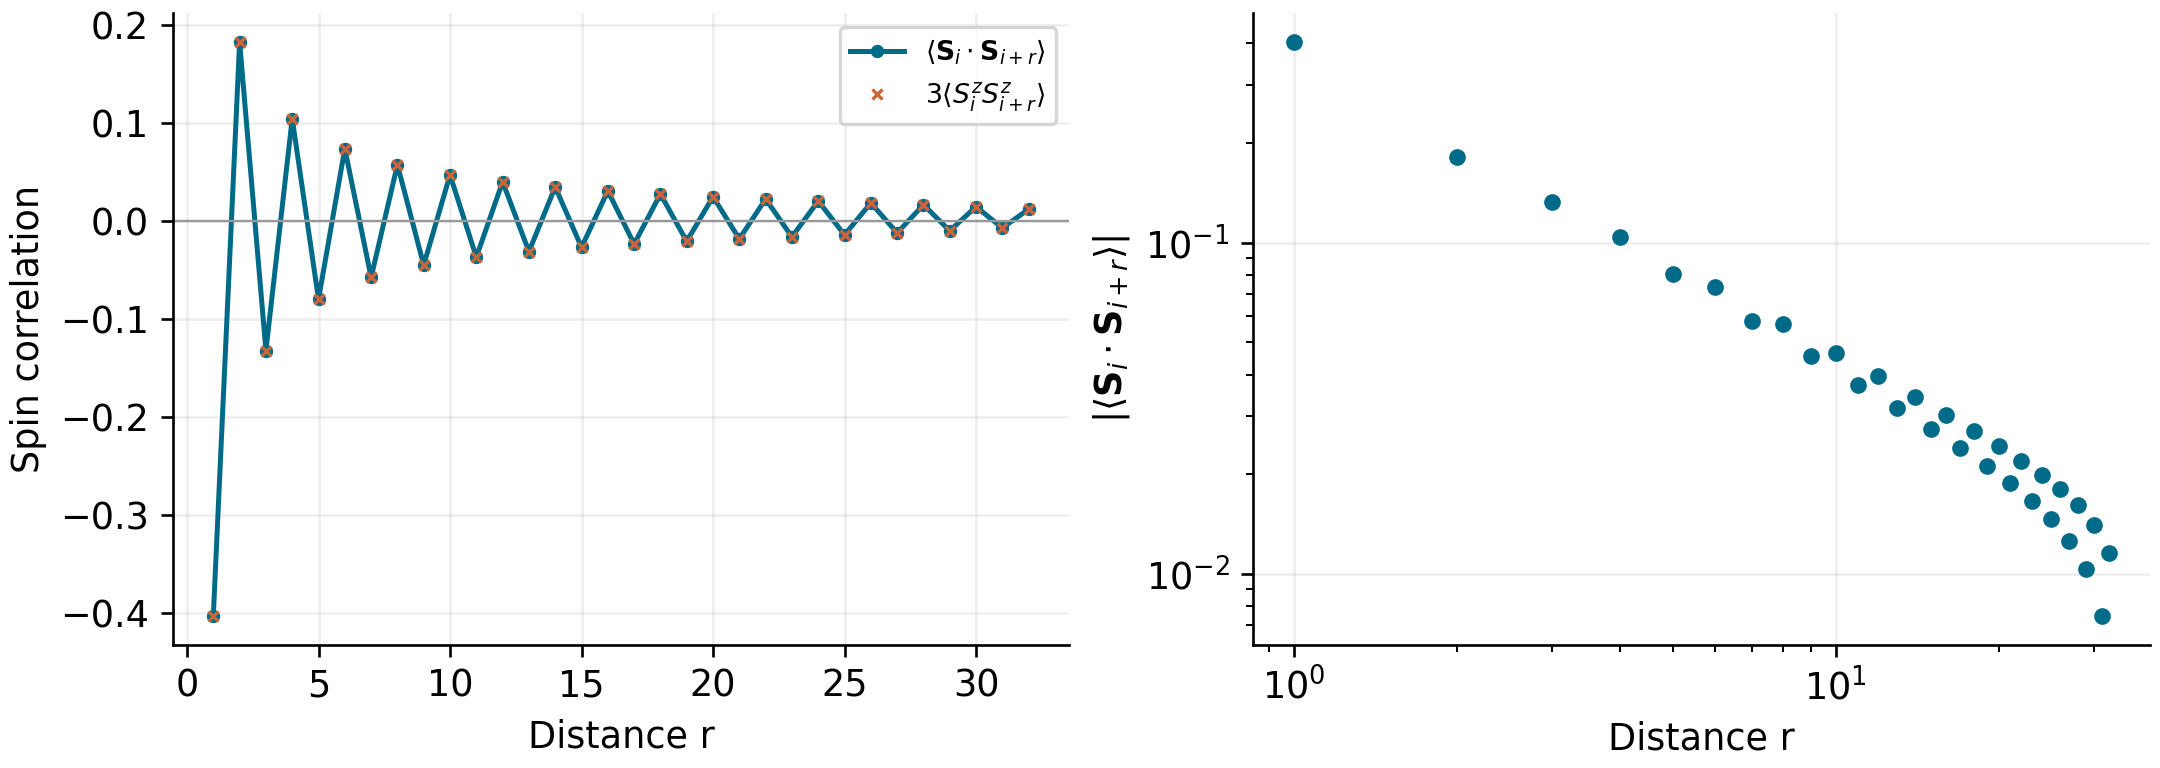
\includegraphics[width=\linewidth]{spin_correlations.png}
\end{center}

\subsection*{结果解释与检查}
奇数距离关联为负、偶数距离为正，关联幅度随距离整体衰减，体现反铁磁关联。
开边界使 $C_{ij}$ 同时依赖 $i,j$；这里展示固定参考格点的结果，
没有假定平移不变性。

数值满足 $C^{zz}(0)=1/4$、$C(0)=3/4$。全链各分量之差小于
$8\times10^{-9}$，局域自旋期望绝对值小于 $4.24\times10^{-11}$，
因此 $C\simeq3C^{zz}$；连通关联
$C_{\mathrm{conn}}^{zz}(i,j)=\avg{S_i^zS_j^z}-\avg{S_i^z}\avg{S_j^z}$
与这里的原始关联几乎相同。

将 $m=64$ 与 $128$ 比较，图中中心关联 $C(r)$ 的最大变化约为
$2.95\times10^{-6}$。完整 $64\times64$ 关联矩阵、逐轮能量和 MPS
已随程序保存，见数据包中的 README。
\end{document}
